\chapter{Recurrent Neural Networks}

Any supervised deep learning algorithm consists of primarily two phases i.e., training and inference. Training is where the network is operated on a dataset consisting of input features, like a speech segment, and the associated correct output, as in this case the word it represents. Once the model has been trained it has the capability to predict the output given a completely new input to an extent of accuracy that is determined the training scheme, the model, the dataset and various other parameters. We now elaborate on the model of a recurrent neural network, illustrate its operation and training mechanism and then explain in detail the model of a Long Short Term Memory Network (LSTM).

\section{RNN Structure}
The Recurrent Neural Network consists of a hidden state that is updated on every new input to the network. The updating of the hidden state of the network is influenced by both the previous state of the network and the new input. The output of the network depends on the hidden state of the network. For a single hidden layer the network can be formulated as follows.
Let the hidden state vector be represented by $\mathbf{h}_t\in\mathbb{R}^{m}$ where $m$ is the dimensionality of the hidden state vector at time step $t$. $\mathbf{x}_t\in\mathbb{R}^{n}$ is the input vector and the output vector is $\mathbf{y}_t\in\mathbb{R}^{k}$ at time step $t$.

\begin{equation}
\mathbf{h}_t = f_W(\mathbf{h}_{t-1},\mathbf{x}_t)
\end{equation}
\begin{equation}
\mathbf{h}_t = tanh(\mathbf{W}_{hh}\mathbf{h}_{t-1} + \mathbf{W}_{xh}\mathbf{x}_t)
\end{equation}
\begin{equation}
\mathbf{y}_t = \mathbf{h}_{hy}\mathbf{h}_t
\end{equation}

\begin{figure}[h]
	\caption{Single Layer RNN}    
    \centering
    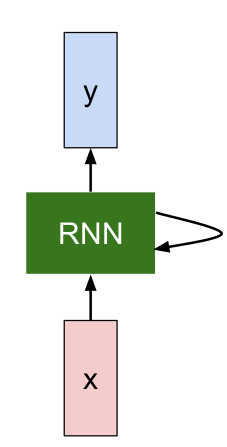
\includegraphics[width=0.1\textwidth]{rnnvanilla}
\end{figure}

The above equations are applied on every new input. The matrices $\mathbf{W}$ represent the connections between the input vector $\mathbf{x}$ and the hidden vector $\mathbf{h}$ as well as the connections between the hidden state and the output vector $\mathbf{y}$. The non-linear function $tanh$ compresses each scalar in the hidden vector to a value between -1 and 1. This non-linearity is crucial to the performance of the network. \\
These connection matrices, more commonly known as weight matrices, are what determine the networks behaviour. The choice of the dimensions of $h$ and the number of hidden layers used determines the capacity of a network to effectively work on the task it is designed for. \\
A good way to visualize the functioning of the network is to observe its behaviour across multiple time steps and and observe the flow of data between the output, the input and within the cell itself. In ~\ref{fig:unroll}, every vertical column of cells represents the same network but at different time instansts.

\begin{figure}[h]
\caption{Unfolded RNN Cell}
\centering
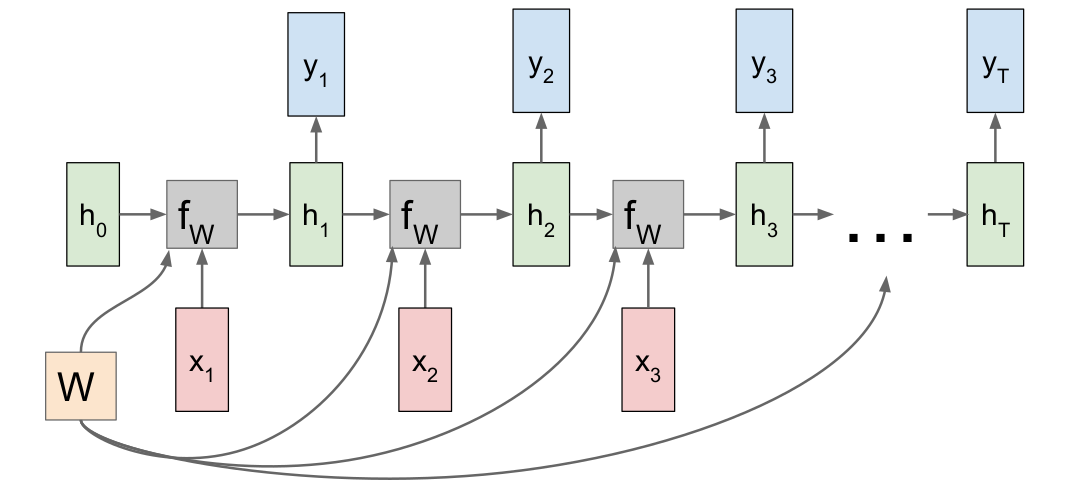
\includegraphics[width=0.8\textwidth]{manyTomany}
\label{fig:unroll}
\end{figure}


A salient point to be noted in recurrent neural networks is that the weight matrices are constant throughout every iteration of the algorithm. This causes some restrictions on what the network is capable of learning:

\begin{enumerate}
    \item The network is poor at learning dependencies between inputs that are separated too far apart as the state of the network tends to slowly forget its past inputs.
    \item During training, the repetition of the matrix causes some terms in the calculation of the training algorithm to explode to infinity or to zero. 
\end{enumerate}
Due to these limitations, a modification of the network known as Long Short Term Memory Networks has been proposed which we will elaborate below.

\section{Long Short Term Memory Networks}
LSTMs were initially introduced by Hochreiter & Schmidhuber in 1997 and through various works was refined into the algorithm used today. An LSTM is a modification of an RNN with additional gates added to it. It consists of three gates that control the flow of information between the input, the hidden state and the output. [ref colahs blog and space]
Let there be:
\begin{enumerate}
    \item Input Connection Weights: $\mathbf{W}_z, \mathbf{W}_s, \mathbf{W}_f, \mathbf{W}_o$ \in $R^{NXM}$ 
    \item Hidden State Weights: $\mathbf{R}_z, \mathbf{R}_s, \mathbf{R}_f, \mathbf{R}_o \in R^{NXN}$
    \item Bias Weights: $\mathbf{b}_z, \mathbf{b}_s, \mathbf{b}_f, \mathbf{b}_o \in R^{N}$
\end{enumerate}
The governing equations of the LSTM update in a time step are as follows:
\begin{equation}
\mathbf{z}^t = \mathbf{W}_z\mathbf{x}^t + \mathbf{R}_z\mathbf{y}^{t-1} + \mathbf{b}_z 
\end{equation}
\begin{equation}
\mathbf{i}^t = \mathbf{W}_i\mathbf{x}^t + \mathbf{R}_i\mathbf{y}^{t-1} + \mathbf{b}_i
\end{equation}
\begin{equation}
\mathbf{i}^t = sigmoid(\mathbf{i}^t)
\end{equation}
\begin{equation}
\mathbf{f}^t = \mathbf{W}_f\mathbf{x}^t + \mathbf{R}_f\mathbf{y}^{t-1} + \mathbf{b}_f
\end{equation}
\begin{equation}
\mathbf{f}^t = sigmoid(\mathbf{f}^t)
\end{equation}
\begin{equation}
\mathbf{c}^t = \mathbf{z}^t\odot\mathbf{i}^t + \mathbf{c}^{t-1}\odot\mathbf{f}^t
\end{equation}
\begin{equation}
\mathbf{o}^t = \mathbf{W}_o\mathbf{x}^t + \mathbf{R}_o\mathbf{y}^{t-1} + \mathbf{b}_o
\end{equation}
\begin{equation}
\mathbf{o}^t = sigmoid(\mathbf{o}^t)
\end{equation}

\begin{equation}
\mathbf{y}^t = tanh(\mathbf{c}^t)\odot\mathbf{o}^t
\end{equation}
$\odot$ represents point-wise multiplication and sigmoid is a logistic function with the following equation 
\[sigmoid(\mathbf{x}) = \frac{1}{1+exp(-\mathbf{x})}\]\\


\begin{figure}[h]
\caption{Graphical representation of an LSTM cell}
\centering
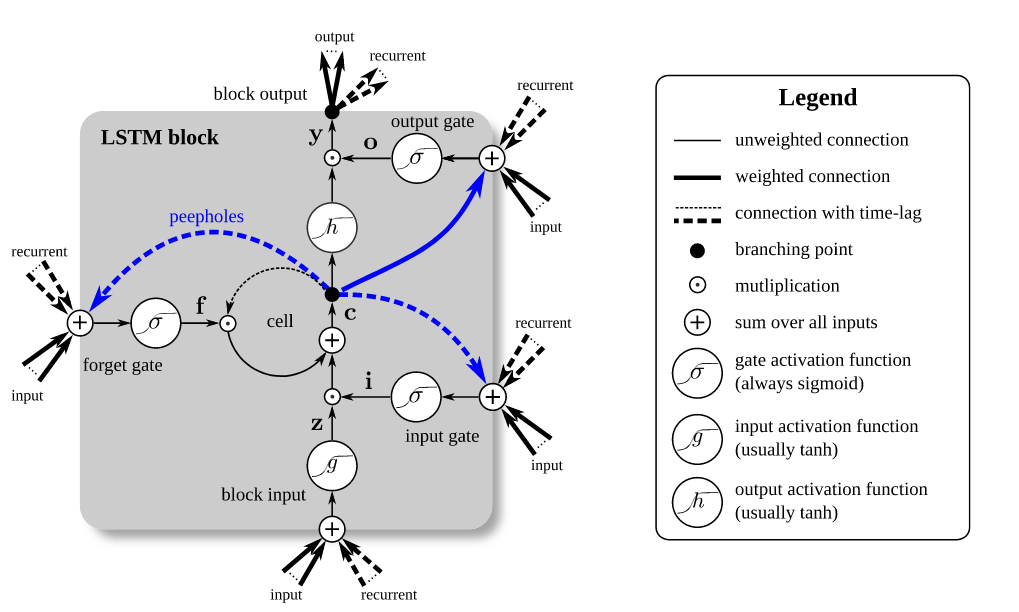
\includegraphics[width=\textwidth]{lstm}
\end{figure}


Each gate serves a purpose: the forget gate controls how much of the previous state is to be retained in the next update, the input gate dictates the influence the new input will have on the state and the output gate controls how much of the output is influence by the hidden state. Due to the addition of these gates, the network has the ability to $remember$ long term dependencies from the input and can solve complex tasks on sequential data.

\subsection{Multi-Layer LSTM}
\begin{figure}[h] 
	\caption{Multi-Layer RNN}    
    \centering
    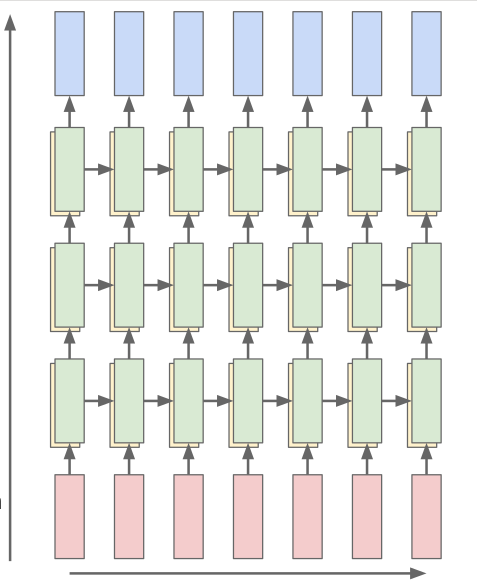
\includegraphics[width=0.25\textwidth]{multi-layer}
\end{figure}
In most state-of-art implementations a single hidden layer isn't used i.e., there isn't just one cell between the input and the output but multiple. This leads to a deep LSTM or a multi-layer LSTM.
\subsection{Google LSTM}


%\section{TIMIT Dataset and Baseline Model}
%In order to compare the results of the various tradeoffs between proposed models and also in order to compare the performance of our final model with others implemented, we need to choose a baseline trained model with optimal performance. The dataset we will be using for this purpose is the TIMIT Acoustic-Phoentic Continuous Speech Corpus. (cite: Garofolo, John S., et al. TIMIT Acoustic-Phonetic Continuous Speech Corpus LDC93S1. Web Download. Philadelphia: Linguistic Data Consortium, 1993.) The dataset contains recordings of 630 speakers covering most of the primary dialects of English, speaking sentences that are phonetically rich. This particular dataset is considered to be a standard for Automatic Speech Recognition Systems and is the dataset of choice for most studies comparing their results with those previously.



